\documentclass{article}

\usepackage{amsmath, amsthm, amssymb, amsfonts}
\usepackage{thmtools}
\usepackage{graphicx}
\usepackage{setspace}
\usepackage{geometry}
\usepackage{float}
\usepackage{hyperref}
\usepackage[utf8]{inputenc}
\usepackage[english]{babel}
\usepackage{framed}
\usepackage[dvipsnames]{xcolor}
\usepackage{tcolorbox}
\usepackage{booktabs}

\newcommand{\HRule}[1]{\rule{\linewidth}{#1}}

\newcommand{\dsanote}[1]{\textbf{[dsa: #1]}}

% ------------------------------------------------------------------------------

\begin{document}

% ------------------------------------------------------------------------------
% Cover Page and ToC
% ------------------------------------------------------------------------------

\title{ \normalsize \textsc{}
		\\ [2.0cm]
		\HRule{1.5pt} \\
		\LARGE \textbf{Parallel and Distributed Computing
		\HRule{2.0pt} \\ [0.6cm] \LARGE{Project Report - MPI Delivery} \vspace*{10\baselineskip}}
		}
\date{}
\author{\textbf{Authors} \\ 
		Carolina Coelho - 99189\\
		Diogo Melita - 99202\\
		Diogo Antunes - 99210}
\maketitle
\newpage

% ------------------------------------------------------------------------------

\section{Introduction}

The goal for this stage is to parallelize the serial version of the \texttt{lifed3d} 
program using MPI.

\section{MPI Approach}

In the \texttt{OpenMP} phase, it was already established which part of the code needed parallelization. 
The main challenge then shifted to parallelizing the computation of successive generations across 
different machines and consolidating the results onto a single machine.

To recall, in the previous stage, the work-sharing was achieved by splitting the
three-deep loop among the different threads. 

\subsection{Data Decomposition}

The initial and arguably crucial step in this stage involved determining how the grid would be 
divided among the various machines. The primary functional approach devised was to partition the 
grid into multiple horizontal slices, with each slice allocated to a different machine. It's 
worth noting that these slices were partitioned to ensure that each had a similar size, thus 
maintaining load balance across the various machines during computation.

This approach led to the decision that each machine would only need to allocate resources for the 
slice it was assigned, effectively reducing the program's memory usage on each machine. Following 
the grid partitioning, the next crucial step was determining how communication between the machines 
would be managed. Given the horizontal partitioning of the grid, each machine would only need to 
communicate with the adjacent machines—specifically, the previous and next machines. During this 
communication, the involved machines would exchange their borders, as these are necessary for 
computing the next generation of border cells.

As each machine only allocates resources for the slice it was assigned to and communicates solely 
with the previous and next machines, it follows that each machine will allocate an additional 
$2 \times n \times n$ cells for the borders of the neighboring slices.

At least two other decompositions were also considered. The first one was one where
the division was done across the x and y axis only and the second one was one where
the division was done across all dimensions. Each machine will have one of the pieces
and for that reason, the less the surface area for the piece, the less communication
there's going to exist. A visualization of the three partitions is provided bellow.

// TODO: add in visualization

Obviously for a fixed number of CPUs, the computation performed in total will essentially
be the same. For division B to be possible, the number must be a product of 2 non-trivial
factors. For division C to be possible, the number must be a product of 3 non-trivial factors.
Let us assume that $p = a \times b \times c$, with $a \ge b \ge c$.

For division A, the expected communication is $2n^2$ cells.
For division B, the division should be done in $a$ in one direction and in $b \times c$
in another direction. The expected communication is $2a \times n + 2b \times c \times n$.
For division C, the expected communication will be $2ab + 2ac + 2bc$. To get a better

Understanding of what this means in practice, let's consider $p=64=4 \times 4 \times 4$.
For division A, the expected communication will be $2n^2$. For division B, the expected
communication will be $4 \times (\frac{n}{4}n)^2 = \frac{n^2}{4}$.
For division C, the expected communication will be $6 \times (\frac{n}{4}\frac{n}{4})^2 = \frac{3n}{128}$.

This shows that the division against more dimensions further reduces communication.
However, it is also clear that the division in more than one dimension is also
much more error-prone. For this reason, our approach was to implement first division
A and if communication proved to be a bottleneck move to more complex grid divisions.

Since instances might be too large to fit into a single machine's memory, each
machine only stores its piece of the map. For each generation, each process will
only compute the statistics for the stored part of the map and at the end the master
root process aggregates all the results and updates the global statistics.

\subsection{Implementation}

The grid will be partitioned in the x-axis and each node will only keep its slice of the grid, the previous and
the next layer.
In the first implementation, at the start of each generation, each node computed
the new values for the current grid (and while doing this, computed the new
statistics), then exchanged with the neighbors the new border values (using the asynchronous
communication primitives \texttt{ISend} and \texttt{IRecv}). At the end of the
exchange the machine-local statistics were aggregated at the root machine (using \texttt{Reduce}).
It should be noted that a single \texttt{ISend} and \texttt{IRecv} are done per layer,
which is possible because the x-y-plane is store contiguously in memory (this isn't possible
for any other plane, in particular for any other data decomposition, the number of calls will
grow with n).

This division already achieved very good speedups, specially for large values of 
$n$. In particular, for the 4 inputs considered, the execution time breakdown can
be found in Figure~\ref{time-breakdown}.
(the raw data is provided in Appendix A, table~\ref{tab:mpi_performance})

\begin{figure}[htbp]
    \centering
    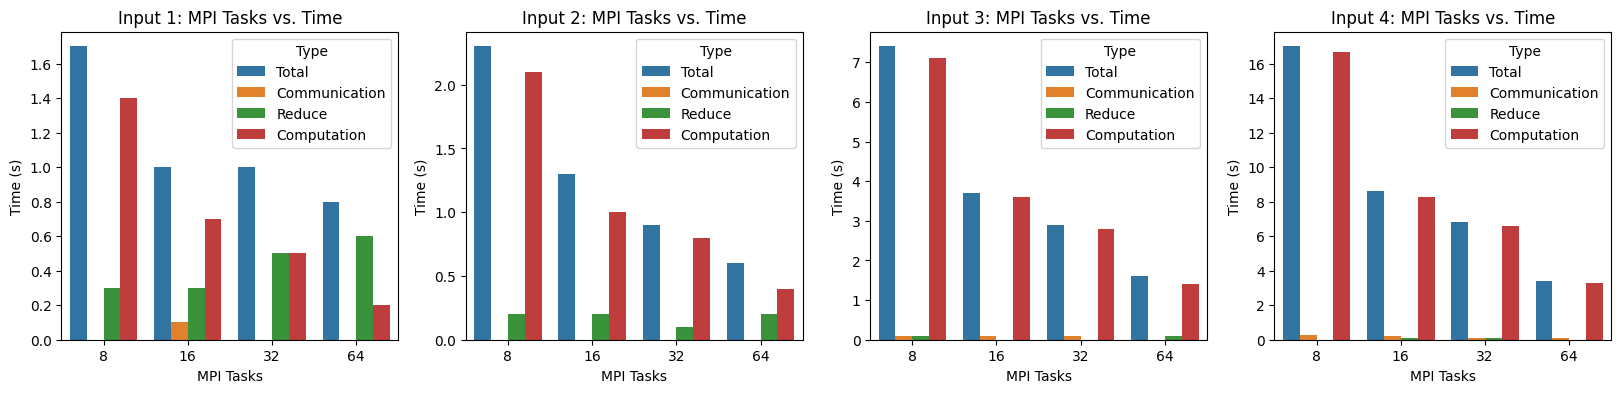
\includegraphics[width=1\textwidth]{img/first-version-breakdown.png}
    \caption{Execution time breakdown for first version}
    \label{time-breakdown}
\end{figure}

As mentioned, computation is the bottleneck across all settings, which implies a small
overhead to parallelization. However, it's
clear that for small values of $n$, the reduction is also problematic. This reduction
step is the moment after the grid update where nodes compute the aggregate value
statistics for the current generation.
The key insight is that this computation can be done while the computation of the
current generation aggregate statistics can be computed in background while
the computation of the new grid state occurs. To do this, \texttt{Reduce} was 
replace by its asynchronous counterpart - \texttt{IReduce}. A small caveat is that
now two local statistics arrays are required - one for the old statistics, upon which
the aggregate value is being computed and one for the new statistics to store
the statistics regarding the new grid that is being computed. With this approach,
each node does the following tasks:

\begin{enumerate}
	\itemsep -0.2em
	\item compute new state of its part of the grid
	\item share borders (using \texttt{ISend} and \texttt{IRecv})
	\item wait for previous reduction (using \texttt{Wait})
	\item root node updates the problem solution
	\item wait for border exchange to complete (using \texttt{WaitAll})
	\item start new reduction (using \texttt{IReduce})
\end{enumerate}

% As previously mentioned, the initial step in transitioning to the simulation phase is to compute the initial 
% statistics of the grid. Given that each machine computes only its local statistics, it becomes necessary to 
% consolidate the statistics of each machine into a single machine. To achieve this, the \texttt{MPI\_Ireduce} function
% was employed. This function was selected for its non-blocking nature, allowing work to continue while communication 
% takes place until the results are required.

% In this stage, since each machine already possesses the initial neighboring cells of its borders at the outset, it 
% can initially compute the next generation of its slice and subsequently update the borders. As a result, the requested 
% reduction results are only needed after border exchanges. Therefore, the \texttt{MPI\_Wait} function is utilized to wait 
% for the completion of the reduction process.
%
% Border exchanging is facilitated through the use of the \texttt{MPI\_Isend} and \texttt{MPI\_Irecv} functions.
% These functions were chosen for their non-blocking nature, allowing work to proceed while communication is underway. 
% In this context, the intermediate work entails updating the grid status by the master machine. Subsequently, the 
% \texttt{MPI\_Waitall} function is employed to await the completion of the border exchange process.
%
% When using the \texttt{MPI\_Isend} and \texttt{MPI\_Irecv} methods, could have be used the communication time to 
% perform the computation of grid values that did not require accessing the border values. However, after conducting 
% several measurements of communication time, it was concluded that it is negligible and does not 
% justify the aforementioned approach.
%
% Following this, it becomes necessary to reduce the statistics computed at the beginning of the simulation. 
% This is accomplished using the \texttt{MPI\_Ireduce} function, as previously mentioned, given that the results 
% are required only after the border exchange has been completed.
%
% It's crucial to highlight that due to the utilization of the \texttt{MPI\_Ireduce} function, each machine must uphold 
% two arrays for the statistics, exchanged before each generation, akin to the grids. This precaution is necessary to 
% prevent potential corruption of statistics, attributable to the non-blocking nature of the function, which permits concurrent 
% work while communication is in progress.

\subsection{Load balancing}

In the current partition of the space, the load for two nodes differs by at most
a single layer. Given the values of $n$ and $p$ considered, it was found that
one always represented a small percentage of the overall workload. The biggest
problem is terms of load balancing was actually found when testing the solution
across labs - the labs machines computing power is not consistent across the cluster
and in this case the homogeneous work division didn't prove to be the best as
the fastest machines had to wait for the slowest in the group. A solution to
this would be to have some dynamic division of work - for example at the end
of each round, every node compared with the neighbors the time it took to do
the update to its region. If the difference was above a threshold, the fastest
neighbor would steal some work. It was considered that this solution was already
out of the scope of the project, so it was not implemented.

\section{Hybrid approach}

Besides the message passing approach, a hybrid approach was also attempted.
As already seen, the communication didn't prove to be much of an overhead, so
no extra speedup was expected from this version. The approach to extending the MPI
solution to a hybrid one resembles the one used to apply OpenMP to the initial
serial version. A team of threads is spawned at the start of MPI instance (using
the \texttt{omp parallel} pragma).
The computation of the new state of the replica's slice is divided among the
threads (using \texttt{omp for}) and all remaining tasks (border exchange and reduction)
are executed only by the master threads, which is achieved using \texttt{omp single}.

\section{Experimental results}

The final solution was benchmarked in RNL lab2 machines against the four public
test provided by the faculty team. The results for the MPI only version 
(\texttt{OMP\_THREAD\_NUM = 1}) is presented in tables \ref{execution-times} and
\ref{speedup}.

\begin{table}[h!]
	\centering
	\begin{tabular}{||c c c c c c||} 
	 \hline
	 Version & \#Nodes & Input 1 & Input 2 & Input 3 & Input 4\\ [0.5ex] 
	 \hline\hline
	 serial & $N/A$ & 13.2 & 20.8 & 72.5 & 168.1 \\ 
	 mpi & 8 & 1.8 & 2.3 & 7.2 & 16.9 \\ 
	 mpi & 16 & 0.9 & 1.2 & 3.9 & 8.5  \\
	 mpi & 32 & 0.7 & 0.9 & 2.9 & 6.8 \\
	 mpi & 64 & 0.4 & 0.5 & 1.5 & 3.7 \\ [1ex] 
	 \hline
	\end{tabular}
	\caption{Times of execution, in seconds, of the serial and parallelized versions of the code.}
	\label{execution-times}
\end{table}

\begin{table}[h!]
	\centering
	\begin{tabular}{||c c c c c||} 
	 \hline
	 \#Nodes & Input 1 & Input 2 & Input 3 & Input 4\\ [0.5ex] 
	 \hline\hline
	 8 & 7.3 & 9 & 10.1 & 9.9 \\ 
	 16 & 14.7 & 17.3 & 18.6 & 19.8  \\
	 32 & 18.9 & 23.1 & 25 & 24.7 \\
	 64 & 33 & 41.6 & 48.6 & 45.4 \\ [1ex] 
	 \hline
	\end{tabular}
	\caption{Speedup achieved with the parallelized versions of the code, comparing to the serial version}
	\label{speedup}
\end{table}

\begin{figure}[htbp]
    \centering
    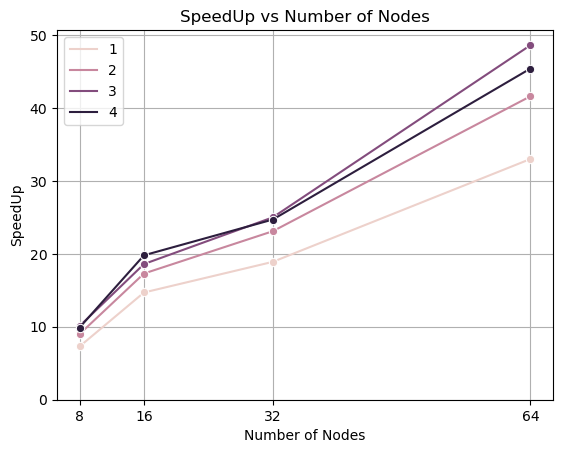
\includegraphics[width=0.5\textwidth]{img/speedup.png}
    \caption{Speedup achieved by the parallelized version when running on different number of nodes.}
    \label{speedup-graph}
\end{figure}

Say that we implemented a version where communication was masked by the computation
The improvement was none or even worse for large n (where this just doesn't apply).
The code and the results are in Appendix B.

\dsanote{Make a plot with the efficiency}
\dsanote{Maybe recall amdal law and check whether it applies}
\dsanote{Gustafson's law}
\dsanote{Measure load balance in machines}

\dsanote{The impact of latency is speedup} -> use experiments with \texttt{-N}

% ist199202@borg:/mnt/cirrus/users/0/2/ist199202/dsa/src/mpi$ srun -n 64 ./life3d-mpi 3 1024 .4 100
% Took: 2.7s
% Communication time: 0.0s
% Reduce time: 0.1s
% Computation time: 2.5s
% 1 99923786 1
% 2 90413714 1
% 3 83137654 1
% 4 77287897 1
% 5 72448825 1
% 6 68444736 1
% 7 65198270 1
% 8 62633412 1
% 9 60611199 1

% ist199202@borg:/mnt/cirrus/users/0/2/ist199202/dsa/src/mpi$ srun -N 64 ./life3d-mpi 3 1024 .4 100
% Took: 8.6s
% Communication time: 0.1s
% Reduce time: 6.2s
% Computation time: 2.4s
% 1 99923786 1
% 2 90413714 1
% 3 83137654 1
% 4 77287897 1
% 5 72448825 1
% 6 68444736 1
% 7 65198270 1
% 8 62633412 1
% 9 60611199 1

% Add MPI_Barrier and one can conclude that it's because some nodes block waiting for others

We didn't do sending with everything else in the background but with small tests
(gen = 10000, n=64), we saw that communication was a bottleneck:

% ist199210@lab3p7:/mnt/cirrus/users/1/0/ist199210/mpi$ srun -n 16  -w lab3p[1,2,4,6] --cpus-per-task=1 --ntasks-per-node=4 ./life3d-mpi 10000 64 0.4 0
% Took: 9.0s
% Reduce+Communication time: 1.2s
% Wait for message exchange time: 0.3s
% Computation time: 7.8s
% 1 81443 62
% 2 24563 24
% 3 20080 1
% 4 19016 1
% 5 17576 1
% 6 16905 1
% 7 15793 1
% 8 15174 1
% 9 14807 1


\section{Results}


\begin{table}[h!]
	\centering
	\begin{tabular}{||c c c c c c c||} 
	 \hline
	 Version & Number of Nodes & Number of Threads & Input 1 & Input 2 & Input 3 & Input 4\\ [0.5ex] 
	 \hline\hline
	 mpi-omp & 16 & 4 & 0.5 & 0.6 & 1.7 & 3.8 \\  [1ex] 
	 \hline
	\end{tabular}
	\caption{Times of execution, in seconds, of the mpi + omp version of the code.}
	\label{times-mpi-omp}
\end{table}

The speedup for small tests is worse than for larger tests, because the communication
is a larger portion of the time spent. We noted that for these scenarios, the
\texttt{Reduce} primitive was one of the major bottlenecks and for that reason,
it was replaced by an asynchronous \texttt{IReduce}. This allowed to mask the
border value communication with the reduce computation. Other strategies could be used
to further reduce computation - compute borders, send border and compute center or 
try another decomposition. Howewver, this communication is already masked with
reduce. Furthermore, for these test sizes, MPI is not the best fit. MPI should
be used for very large tests that do not fit into the memory of a single machine.
For this reason, further adding changes to the code would be trying to optimize
for something that is not the target use case and for that reason, it was not done.

It should be noted that for large test cases ($n=1024$), communicatino was found
to be a very small fraction of the time, so the bottleneck really was computation power.

A note on load balancing and the heteregenoriy of the cluster.

\newpage

\begin{table}[htbp]
  \centering
  \label{tab:mpi_performance}
  \begin{tabular}{lcccc}
    \toprule
    \textbf{Number of tasks} & \textbf{Total time (s)} & \textbf{Communication (s)} & \textbf{Reduce (s)} & \textbf{Computation (s)} \\
    \midrule
    \textbf{Input 1} & & & & \\
    8 MPI Tasks & 1.7 & 0.0 & 0.3 & 1.4 \\
    16 MPI Tasks & 1.0 & 0.1 & 0.3 & 0.7 \\
    32 MPI Tasks & 1.0 & 0.0 & 0.5 & 0.5 \\
    64 MPI Tasks & 0.8 & 0.0 & 0.6 & 0.2 \\
    \midrule
    \textbf{Input 2} & & & & \\
    8 MPI Tasks & 2.3 & 0.0 & 0.2 & 2.1 \\
    16 MPI Tasks & 1.3 & 0.0 & 0.2 & 1.0 \\
    32 MPI Tasks & 0.9 & 0.0 & 0.1 & 0.8 \\
    64 MPI Tasks & 0.6 & 0.0 & 0.2 & 0.4 \\
    \midrule
    \textbf{Input 3} & & & & \\
    8 MPI Tasks & 7.4 & 0.1 & 0.1 & 7.1 \\
    16 MPI Tasks & 3.7 & 0.1 & 0.0 & 3.6 \\
    32 MPI Tasks & 2.9 & 0.1 & 0.0 & 2.8 \\
    64 MPI Tasks & 1.6 & 0.0 & 0.1 & 1.4 \\
    \midrule
    \textbf{Input 4} & & & & \\
    8 MPI Tasks & 17.0 & 0.3 & 0.0 & 16.7 \\
    16 MPI Tasks & 8.6 & 0.2 & 0.1 & 8.3 \\
    32 MPI Tasks & 6.8 & 0.1 & 0.1 & 6.6 \\
    64 MPI Tasks & 3.4 & 0.1 & 0.0 & 3.3 \\
    \bottomrule
  \end{tabular}
  \caption{First version execution time breakdown}
\end{table}

\begin{table}[htbp]
  \centering
  \caption{MPI Performance Summary}
  \label{tab:mpi_performance}
  \begin{tabular}{lcccc}
    \toprule
    \textbf{Task} & \textbf{MPI Tasks} & \textbf{Took (s)} \\
    \midrule
    \textbf{2} & & \\
    8 MPI Tasks & 1.7 \\
    16 MPI Tasks & 1.1 \\
    32 MPI Tasks & 0.7 \\
    64 MPI Tasks & 0.5 \\
    \midrule
    \textbf{a3} & & \\
    8 MPI Tasks & 2.2 \\
    16 MPI Tasks & 1.7 \\
    32 MPI Tasks & 0.9 \\
    64 MPI Tasks & 0.5 \\
    \midrule
    \textbf{a4} & & \\
    8 MPI Tasks & 7.3 \\
    16 MPI Tasks & 5.7 \\
    32 MPI Tasks & 2.9 \\
    64 MPI Tasks & 1.5 \\
    \midrule
    \textbf{a5} & & \\
    8 MPI Tasks & 17.1 \\
    16 MPI Tasks & 13.5 \\
    32 MPI Tasks & 7.3 \\
    64 MPI Tasks & 3.4 \\
    \bottomrule
  \end{tabular}
\end{table}


    for (int32_t gen = 0; gen < max_gen; gen++) {
      computation_time = -MPI_Wtime();

        for (int32_t y = 0; y < n; y++) {
          for (int32_t z = 0; z < n; z++) {
            new_val = next_inhabitant(1, y, z, n, old);
            new[1][y][z] = new_val;
            population_local[new_val]++;
            // fprintf(stderr, "next_inhabitant(%d, %d, %d, %d, grid) = %d\n", x, y,
            //         z, n, new[x][y][z]);
          }
        }

        if (height > 1) {
        for (int32_t y = 0; y < n; y++) {
          for (int32_t z = 0; z < n; z++) {
            new_val = next_inhabitant(height, y, z, n, old);
            new[height][y][z] = new_val;
            population_local[new_val]++;
            // fprintf(stderr, "next_inhabitant(%d, %d, %d, %d, grid) = %d\n", x, y,
            //         z, n, new[x][y][z]);
          }
        }
        }

      computation_time += MPI_Wtime();
      total_computation_time += computation_time;

          //fprintf(stderr, "[%d] Computation time: %.1fs\n", me, computation_time);
        memcpy(top, &(new[1][0][0]), n2);
        if (height > 1) memcpy(bottom, &(new[height][0][0]), n2);

        //(stderr, "[%d] Sending and receiving stuff\n", me);
        MPI_Isend(top, n*n, MPI_CHAR, neighbour_prev, TAG_PREV, comm, requests);
        MPI_Irecv(&(new[height+1][0][0]), n*n, MPI_CHAR, neighbour_next, TAG_PREV, comm, requests+2);

        if (height > 1) MPI_Isend(bottom, n*n, MPI_CHAR, neighbour_next, TAG_NEXT, comm, requests+1);
        else MPI_Isend(top, n*n, MPI_CHAR, neighbour_next, TAG_NEXT, comm, requests+1);

        MPI_Irecv(&(new[0][0][0]), n*n, MPI_CHAR, neighbour_prev, TAG_NEXT, comm, requests+3);

        //fprintf(stderr, "[%d] Sending and receiving stuff @ WaitAll\n", me);
      for (int32_t x = 2; x <= height-1; x++) {
        for (int32_t y = 0; y < n; y++) {
          for (int32_t z = 0; z < n; z++) {
            new_val = next_inhabitant(x, y, z, n, old);
            new[x][y][z] = new_val;
            population_local[new_val]++;
            // fprintf(stderr, "next_inhabitant(%d, %d, %d, %d, grid) = %d\n", x, y,
            //         z, n, new[x][y][z]);
          }
        }
      }

        MPI_Wait(&request_reduce, &status_reduce);
        if (me == 0) {
          for (int i = 0; i <= N_SPECIES; i++) {
            if (max_population[i] < population[i]) {
              max_population[i] = population[i];
              peak_gen[i] = gen;
            }
          }
        }

        memset(population_local_old, 0, sizeof(uint64_t) * (N_SPECIES + 1));

        MPI_Waitall(4, requests, status);

        tmp = old;
        old = new;
        new = tmp;

        population_local_tmp = population_local_old;
        population_local_old = population_local;
        population_local = population_local_tmp;

        //fprintf(stderr, "[%d] Computing stats\n", me);
        // No need for barrier, because all must say something for reduce
        reduce_time = -MPI_Wtime();
        MPI_Ireduce(population_local_old, population, N_SPECIES+1, MPI_UNSIGNED_LONG, MPI_SUM, 0, comm, &request_reduce);
        reduce_time += MPI_Wtime();
        total_reduce_time += reduce_time;
      }
  MPI_Wait(&request_reduce, &status_reduce);


% ------------------------------------------------------------------------------
% Reference and Cited Works
% ------------------------------------------------------------------------------

\bibliographystyle{IEEEtran}
% \bibliography{References.bib}

% ------------------------------------------------------------------------------

\end{document}
